\begin{pastexam}[label={px:ncku-109-ee-ds-06}]{成大電機所 109 學年度 第 6 題}
（問答；25 分）

Consider a sequence of keys：27, 49, 17, 20, 61, 23, 92, 33, 77, 11, 31.
\begin{enumerate}[label=(\alph*)]
\item Draw, \textbf{step by step} (showing clearly the type of rotation used), the result of
inserting these keys into an empty AVL tree. \quad (20 points)
\item Write down the inorder sequence of the AVL tree in (a). \quad (5 points)
\end{enumerate}
\end{pastexam}

\begin{pastsoln}
\textbf{(a)} 照資結書第~10.2.3~節的插入：先照 BST 插入，再從新節點往根找第一個平衡因子
（左子樹高 $-$ 右子樹高）變成 $\pm 2$ 的節點 $A$，依新節點在 $A$ 的哪一邊做 LL、RR（單旋轉）或
LR、RL（雙旋轉）。 這組資料共旋轉三次：插入 $23$ 時 RR、插入 $92$ 時 RR、插入 $31$ 時 LL。 圖中
灰色是這一步新插入的節點。

\textbf{插入 27、49、17、20、61}：都不失衡。
\begin{center}
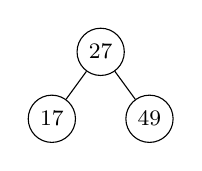
\begin{tikzpicture}[baseline=(current bounding box.center),every node/.style={circle,draw,minimum size=6mm,inner sep=0pt,font=\footnotesize}]
\node[] (n17) at (0.00,-0.85) {17};
\node[] (n27) at (0.62,0.00) {27};
\node[] (n49) at (1.24,-0.85) {49};
\draw (n27) -- (n17);
\draw (n27) -- (n49);
\end{tikzpicture}\qquad
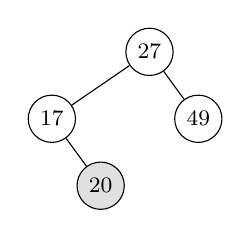
\begin{tikzpicture}[baseline=(current bounding box.center),every node/.style={circle,draw,minimum size=6mm,inner sep=0pt,font=\footnotesize}]
\node[] (n17) at (0.00,-0.85) {17};
\node[fill=black!12] (n20) at (0.62,-1.70) {20};
\node[] (n27) at (1.24,0.00) {27};
\node[] (n49) at (1.86,-0.85) {49};
\draw (n17) -- (n20);
\draw (n27) -- (n17);
\draw (n27) -- (n49);
\end{tikzpicture}\qquad
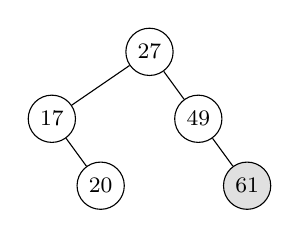
\begin{tikzpicture}[baseline=(current bounding box.center),every node/.style={circle,draw,minimum size=6mm,inner sep=0pt,font=\footnotesize}]
\node[] (n17) at (0.00,-0.85) {17};
\node[] (n20) at (0.62,-1.70) {20};
\node[] (n27) at (1.24,0.00) {27};
\node[] (n49) at (1.86,-0.85) {49};
\node[fill=black!12] (n61) at (2.48,-1.70) {61};
\draw (n17) -- (n20);
\draw (n49) -- (n61);
\draw (n27) -- (n17);
\draw (n27) -- (n49);
\end{tikzpicture}
\end{center}

\textbf{插入 23}：$23 > 17$、$23 > 20$，放在 $20$ 的右邊。 $17$ 的左子樹高 $0$、右子樹高 $2$，平衡
因子 $-2$，新節點在 $17$ 的右子節點的右子樹，是 \textbf{RR}：對 $17$ 左旋，$20$ 升上來。
\begin{center}
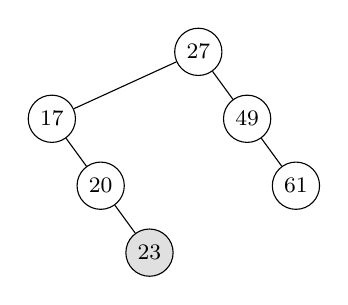
\begin{tikzpicture}[baseline=(current bounding box.center),every node/.style={circle,draw,minimum size=6mm,inner sep=0pt,font=\footnotesize}]
\node[] (n17) at (0.00,-0.85) {17};
\node[] (n20) at (0.62,-1.70) {20};
\node[fill=black!12] (n23) at (1.24,-2.55) {23};
\node[] (n27) at (1.86,0.00) {27};
\node[] (n49) at (2.48,-0.85) {49};
\node[] (n61) at (3.10,-1.70) {61};
\draw (n20) -- (n23);
\draw (n17) -- (n20);
\draw (n49) -- (n61);
\draw (n27) -- (n17);
\draw (n27) -- (n49);
\end{tikzpicture}
\quad$\Longrightarrow$\quad
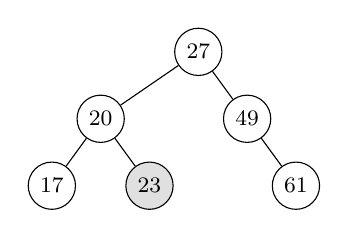
\begin{tikzpicture}[baseline=(current bounding box.center),every node/.style={circle,draw,minimum size=6mm,inner sep=0pt,font=\footnotesize}]
\node[] (n17) at (0.00,-1.70) {17};
\node[] (n20) at (0.62,-0.85) {20};
\node[fill=black!12] (n23) at (1.24,-1.70) {23};
\node[] (n27) at (1.86,0.00) {27};
\node[] (n49) at (2.48,-0.85) {49};
\node[] (n61) at (3.10,-1.70) {61};
\draw (n20) -- (n17);
\draw (n20) -- (n23);
\draw (n49) -- (n61);
\draw (n27) -- (n20);
\draw (n27) -- (n49);
\end{tikzpicture}
\end{center}

\textbf{插入 92}：放在 $61$ 的右邊。 $49$ 的平衡因子 $-2$，\textbf{RR}：對 $49$ 左旋，$61$ 升上來。
\begin{center}
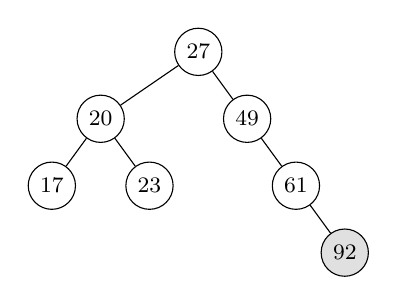
\begin{tikzpicture}[baseline=(current bounding box.center),every node/.style={circle,draw,minimum size=6mm,inner sep=0pt,font=\footnotesize}]
\node[] (n17) at (0.00,-1.70) {17};
\node[] (n20) at (0.62,-0.85) {20};
\node[] (n23) at (1.24,-1.70) {23};
\node[] (n27) at (1.86,0.00) {27};
\node[] (n49) at (2.48,-0.85) {49};
\node[] (n61) at (3.10,-1.70) {61};
\node[fill=black!12] (n92) at (3.72,-2.55) {92};
\draw (n20) -- (n17);
\draw (n20) -- (n23);
\draw (n61) -- (n92);
\draw (n49) -- (n61);
\draw (n27) -- (n20);
\draw (n27) -- (n49);
\end{tikzpicture}
\quad$\Longrightarrow$\quad
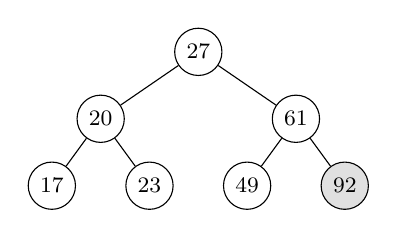
\begin{tikzpicture}[baseline=(current bounding box.center),every node/.style={circle,draw,minimum size=6mm,inner sep=0pt,font=\footnotesize}]
\node[] (n17) at (0.00,-1.70) {17};
\node[] (n20) at (0.62,-0.85) {20};
\node[] (n23) at (1.24,-1.70) {23};
\node[] (n27) at (1.86,0.00) {27};
\node[] (n49) at (2.48,-1.70) {49};
\node[] (n61) at (3.10,-0.85) {61};
\node[fill=black!12] (n92) at (3.72,-1.70) {92};
\draw (n20) -- (n17);
\draw (n20) -- (n23);
\draw (n61) -- (n49);
\draw (n61) -- (n92);
\draw (n27) -- (n20);
\draw (n27) -- (n61);
\end{tikzpicture}
\end{center}

\textbf{插入 33、77、11}：$33$ 放在 $49$ 的左邊，$77$ 放在 $92$ 的左邊，$11$ 放在 $17$ 的左邊。 每次
沿路節點的平衡因子都在 $-1$ 到 $1$ 之間，不必旋轉（插入 $77$ 後根的平衡因子是 $2 - 3 = -1$，
插入 $11$ 後變成 $0$）。
\begin{center}
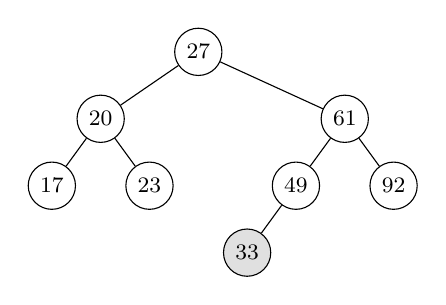
\begin{tikzpicture}[baseline=(current bounding box.center),every node/.style={circle,draw,minimum size=6mm,inner sep=0pt,font=\footnotesize}]
\node[] (n17) at (0.00,-1.70) {17};
\node[] (n20) at (0.62,-0.85) {20};
\node[] (n23) at (1.24,-1.70) {23};
\node[] (n27) at (1.86,0.00) {27};
\node[fill=black!12] (n33) at (2.48,-2.55) {33};
\node[] (n49) at (3.10,-1.70) {49};
\node[] (n61) at (3.72,-0.85) {61};
\node[] (n92) at (4.34,-1.70) {92};
\draw (n20) -- (n17);
\draw (n20) -- (n23);
\draw (n49) -- (n33);
\draw (n61) -- (n49);
\draw (n61) -- (n92);
\draw (n27) -- (n20);
\draw (n27) -- (n61);
\end{tikzpicture}\qquad
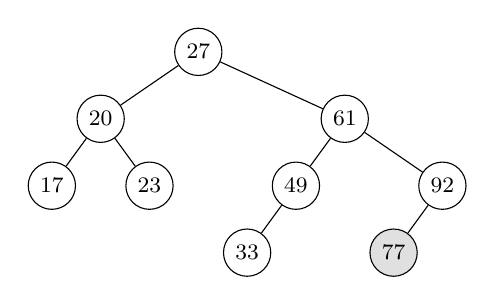
\begin{tikzpicture}[baseline=(current bounding box.center),every node/.style={circle,draw,minimum size=6mm,inner sep=0pt,font=\footnotesize}]
\node[] (n17) at (0.00,-1.70) {17};
\node[] (n20) at (0.62,-0.85) {20};
\node[] (n23) at (1.24,-1.70) {23};
\node[] (n27) at (1.86,0.00) {27};
\node[] (n33) at (2.48,-2.55) {33};
\node[] (n49) at (3.10,-1.70) {49};
\node[] (n61) at (3.72,-0.85) {61};
\node[fill=black!12] (n77) at (4.34,-2.55) {77};
\node[] (n92) at (4.96,-1.70) {92};
\draw (n20) -- (n17);
\draw (n20) -- (n23);
\draw (n49) -- (n33);
\draw (n92) -- (n77);
\draw (n61) -- (n49);
\draw (n61) -- (n92);
\draw (n27) -- (n20);
\draw (n27) -- (n61);
\end{tikzpicture}
\end{center}
\begin{center}
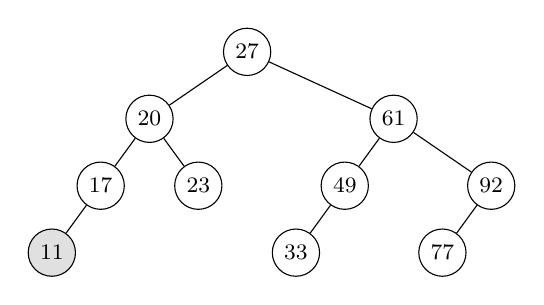
\begin{tikzpicture}[baseline=(current bounding box.center),every node/.style={circle,draw,minimum size=6mm,inner sep=0pt,font=\footnotesize}]
\node[fill=black!12] (n11) at (0.00,-2.55) {11};
\node[] (n17) at (0.62,-1.70) {17};
\node[] (n20) at (1.24,-0.85) {20};
\node[] (n23) at (1.86,-1.70) {23};
\node[] (n27) at (2.48,0.00) {27};
\node[] (n33) at (3.10,-2.55) {33};
\node[] (n49) at (3.72,-1.70) {49};
\node[] (n61) at (4.34,-0.85) {61};
\node[] (n77) at (4.96,-2.55) {77};
\node[] (n92) at (5.58,-1.70) {92};
\draw (n17) -- (n11);
\draw (n20) -- (n17);
\draw (n20) -- (n23);
\draw (n49) -- (n33);
\draw (n92) -- (n77);
\draw (n61) -- (n49);
\draw (n61) -- (n92);
\draw (n27) -- (n20);
\draw (n27) -- (n61);
\end{tikzpicture}
\end{center}

\textbf{插入 31}：$31 > 27$、$< 61$、$< 49$、$< 33$，放在 $33$ 的左邊。 往上檢查：$33$ 是 $+1$，
$49$ 的左子樹高 $2$、右子樹高 $0$，平衡因子 $+2$。 新節點在 $49$ 的左子節點的左子樹，是
\textbf{LL}：對 $49$ 右旋，$33$ 升上來。 旋轉後這棵子樹的高度回到插入前的 $2$，上面的 $61$、$27$
不受影響。
\begin{center}
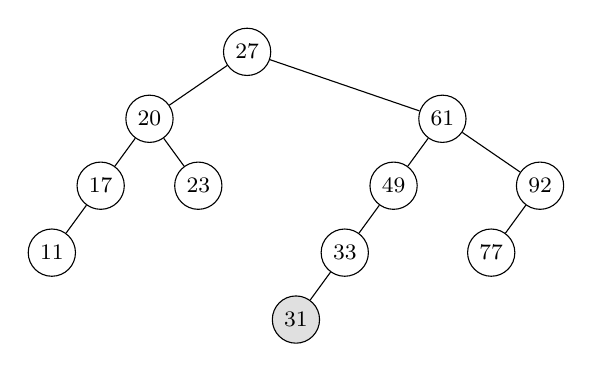
\begin{tikzpicture}[baseline=(current bounding box.center),every node/.style={circle,draw,minimum size=6mm,inner sep=0pt,font=\footnotesize}]
\node[] (n11) at (0.00,-2.55) {11};
\node[] (n17) at (0.62,-1.70) {17};
\node[] (n20) at (1.24,-0.85) {20};
\node[] (n23) at (1.86,-1.70) {23};
\node[] (n27) at (2.48,0.00) {27};
\node[fill=black!12] (n31) at (3.10,-3.40) {31};
\node[] (n33) at (3.72,-2.55) {33};
\node[] (n49) at (4.34,-1.70) {49};
\node[] (n61) at (4.96,-0.85) {61};
\node[] (n77) at (5.58,-2.55) {77};
\node[] (n92) at (6.20,-1.70) {92};
\draw (n17) -- (n11);
\draw (n20) -- (n17);
\draw (n20) -- (n23);
\draw (n33) -- (n31);
\draw (n49) -- (n33);
\draw (n92) -- (n77);
\draw (n61) -- (n49);
\draw (n61) -- (n92);
\draw (n27) -- (n20);
\draw (n27) -- (n61);
\end{tikzpicture}
\end{center}
\begin{center}
$\Longrightarrow$\quad
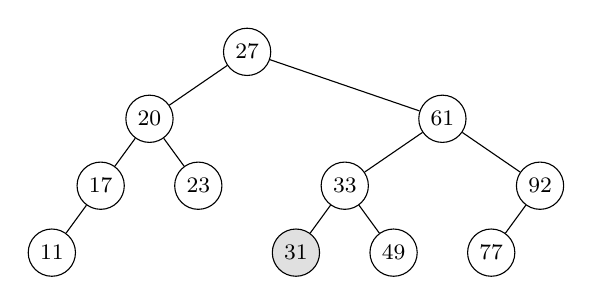
\begin{tikzpicture}[baseline=(current bounding box.center),every node/.style={circle,draw,minimum size=6mm,inner sep=0pt,font=\footnotesize}]
\node[] (n11) at (0.00,-2.55) {11};
\node[] (n17) at (0.62,-1.70) {17};
\node[] (n20) at (1.24,-0.85) {20};
\node[] (n23) at (1.86,-1.70) {23};
\node[] (n27) at (2.48,0.00) {27};
\node[fill=black!12] (n31) at (3.10,-2.55) {31};
\node[] (n33) at (3.72,-1.70) {33};
\node[] (n49) at (4.34,-2.55) {49};
\node[] (n61) at (4.96,-0.85) {61};
\node[] (n77) at (5.58,-2.55) {77};
\node[] (n92) at (6.20,-1.70) {92};
\draw (n17) -- (n11);
\draw (n20) -- (n17);
\draw (n20) -- (n23);
\draw (n33) -- (n31);
\draw (n33) -- (n49);
\draw (n92) -- (n77);
\draw (n61) -- (n33);
\draw (n61) -- (n92);
\draw (n27) -- (n20);
\draw (n27) -- (n61);
\end{tikzpicture}
\end{center}
最後的 AVL 樹就是上面最後一張圖：根 $27$；左子樹 $20(17(11), 23)$；右子樹
$61(33(31, 49), 92(77))$。 檢查每個節點的平衡因子：$27$ 是 $3 - 3 = 0$，$20$ 是 $+1$，$17$ 是 $+1$，
$61$ 是 $0$，$33$ 是 $0$，$92$ 是 $+1$，其餘樹葉是 $0$。

\textbf{(b)} BST 的中序走訪一定是由小到大（資結書定理~9.1），旋轉不改變中序：
\[
11,\ 17,\ 20,\ 23,\ 27,\ 31,\ 33,\ 49,\ 61,\ 77,\ 92 .
\]
\end{pastsoln}
